\documentclass[11pt]{article}
\usepackage[letterpaper,margin=1in]{geometry}
\usepackage[T1]{fontenc}
\usepackage{lmodern}
\usepackage{tikz}
\usetikzlibrary{arrows.meta}
\pdftrailerid{}
\pdfsuppressptexinfo=15
\usepackage{amsmath,amssymb,amsthm,mathtools}
\usepackage{microtype}
\usepackage{enumitem}
\usepackage{needspace}
\usepackage{xcolor}
\usepackage[colorlinks=true,linkcolor=blue!45!black,citecolor=blue!45!black,urlcolor=blue!45!black]{hyperref}
\usepackage{bookmark}
\hypersetup{pdftitle={Integral and fractional expectation thresholds are equivalent},pdfauthor={OpenAI},bookmarksdepth=2}
\urlstyle{same}
\newcommand{\F}{\mathcal F}
\newcommand{\G}{\mathcal G}
\newcommand{\E}{\mathbb E}
\renewcommand{\P}{\mathbb P}
\newcommand{\N}{\mathbb N}
\newcommand{\R}{\mathbb R}
\newtheorem{theorem}{Theorem}[section]
\newtheorem{lemma}[theorem]{Lemma}
\newtheorem{proposition}[theorem]{Proposition}
\newtheorem{corollary}[theorem]{Corollary}
\theoremstyle{remark}
\newtheorem{remark}[theorem]{Remark}
\numberwithin{equation}{section}
\setlength{\emergencystretch}{1.5em}
\title{Integral and fractional expectation thresholds are equivalent}
\author{OpenAI}
\date{September 23, 2026}
\begin{document}
\maketitle
\begin{abstract}
We prove Talagrand's conjecture that integral and fractional expectation
thresholds are within a universal constant factor, with the same covering
budget.
\end{abstract}
\section{Introduction}

Expectation thresholds measure how cheaply an increasing family can be
covered by elementary containment events. Their fractional relaxation
allows a member to be covered by a total weight of one, distributed
among its subsets. Talagrand conjectured that this relaxation changes
the expectation threshold by at most a universal factor
\cite[Conjecture~6.3]{Talagrand2010}. We prove this conjecture.

Let $X$ be a finite nonempty set and let $\F$ be a nonempty proper
increasing subfamily of $2^X$. For a family $\G\subseteq2^X$ and a
function $g:2^X\to[0,1]$, define
\[
 \langle\G\rangle
 =\{H\subseteq X:\exists S\in\G,\ S\subseteq H\},
 \qquad
 c_p(\G)=\sum_{S\in\G}p^{|S|},
\]
and
\[
 \langle g\rangle
 =\left\{H\subseteq X:\sum_{S\subseteq H}g(S)\ge1\right\},
 \qquad
 w(g,p)=\sum_{S\subseteq X}g(S)p^{|S|}.
\]
Throughout, $p\in[0,1]$ and $p^0=1$, including when $p=0$.
Thus a cover supplies, inside each member of $\F$, at least one
generator $S\in\G$. If $X_p$ includes the elements of $X$ independently
with probability $p$, the cost of that generator is
$\mathbb P(S\subseteq X_p)=p^{|S|}$.
We say that $\F$ is \emph{$p$-small} if there is a family $\G$ with
$\F\subseteq\langle\G\rangle$ and $c_p(\G)\le1/2$.
Its integral and fractional expectation thresholds are
\begin{align*}
 q(\F)
 &=\max\{p\in[0,1]:\F\text{ is }p\text{-small}\},\\
 q_f(\F)
 &=\max\{p\in[0,1]:\exists g:2^X\to[0,1],
       \F\subseteq\langle g\rangle,
       \ w(g,p)\le1/2\}.
\end{align*}
In particular, $q(\F)\le q_f(\F)$, by taking $g$ to be the indicator
of an integral cover.

These maxima are well-defined. Since $\varnothing\notin\F$, both
feasible parameter sets contain zero. Integral feasibility is a finite
union of closed subsets of $[0,1]$. Fractional feasibility is the
projection of the compact set of pairs $(p,g)$ satisfying the displayed
constraints in $[0,1]\times[0,1]^{2^X}$.

\Needspace{9\baselineskip}
\begin{theorem}\label{thm:main}
For every finite nonempty $X$ and every nonempty proper increasing
family $\F\subseteq2^X$,
\[
 q_f(\F)\le25\cdot512^4\,q(\F).
\]
Both thresholds use the budget $1/2$. The constant is independent of
$|X|$, the sizes of the minimal members of $\F$, and the support of
the fractional cover.
\end{theorem}

The conclusion preserves the covering budget: every fractional cover of
cost at most $1/2$ at a parameter $r$ admits an integral cover of cost at
most $1/2$ at $r/(25\cdot512^4)$.

\subsection{Thresholds, selectors, and earlier comparisons}

Expectation thresholds arose in the study of when a random set first
has a prescribed increasing property. Let $p_c(\F)$ denote the unique
parameter for which $\mathbb P(X_p\in\F)=1/2$. A union bound applied to
an integral cover gives $q(\F)\le p_c(\F)$; taking expectations in a
fractional cover gives $q_f(\F)\le p_c(\F)$ as well.
Kahn and Kalai~\cite{KahnKalai2007} conjectured the upper bound
$p_c(\F)=O(q(\F)\log(2|X|))$.
Frankston, Kahn, Narayanan, and Park~\cite{FKNP2021}, building on the
sunflower methods of Alweiss, Lovett, Wu, and Zhang~\cite{ALWZ2021},
proved the fractional bound
\[
 p_c(\F)=O(q_f(\F)\log\ell),
 \qquad
 \ell=\max\{2,\max\{|H|:H\text{ is a minimal member of }\F\}\}.
\]
Park and Pham~\cite{ParkPham2024threshold} proved the corresponding
bound with $q$ in place of $q_f$, resolving the Kahn--Kalai conjecture.
These theorems estimate the random-set threshold. Talagrand's comparison
asks whether fractional certificates themselves admit integral
replacements at a constant loss.

Early results obtained such replacements by exploiting the structure
of the sets with positive fractional weight. Talagrand settled the case
of singleton sets~\cite[Section~6]{Talagrand2010}; DeMarco and
Kahn~\cite{DeMarcoKahn2015} treated clique-counting certificates, and
Frankston, Kahn, and Park~\cite{FrankstonKahnPark2022} treated arbitrary
weights on pairs. Fischer and Person extended these methods to nearly
linear uniform hypergraphs~\cite{FischerPerson2025} and further clique
cases~\cite{FischerPerson2025further}. They also proved the comparison
with high probability for constant weights on random uniform supports
\cite{FischerPerson2026random}.

Selector processes supply a different route: they seek a member whose
assigned vertex mass is substantially captured by a random subset.
Park and Pham proved Talagrand's selector-process conjecture
\cite{ParkPham2024selector}, and Bednorz, Martynek, and
Meller~\cite{BMM2022} gave a proof using truncated weights.
Dubroff, Kahn, and Park~\cite[Theorem~1.2]{DKP2024} used selector
estimates to round any fractional cover whose positive coefficients
occur only on sets of cardinality at most $t$, with a loss depending on
$t$. Pham sharpened this loss to $O(\log(2t))$
\cite[arXiv version~1, Theorem~1.2]{Pham2024}.
Here $t$ bounds the cardinalities of the weighted sets, not their number
or the sizes of the minimal members of $\F$. For example, for
$1\le k\le|X|$, the family $\{H\subseteq X:|H|\ge k\}$ has the
fractional cover $g(\{x\})=1/k$, zero elsewhere: its weighted sets are
singletons, while its minimal members have cardinality $k$.

Fischer and Person's sampling argument for sufficiently large sets
\cite[Theorem~10]{FischerPerson2025}, combined with Pham's logarithmic
rounding bound, gives a loss of order $\log\log(4|X|)$. This consequence
is recorded in the expanded version of Pham's paper
\cite[Corollary~1.8]{Pham2026}. More recently, Park
\cite[Theorem~1.2]{Park2026} obtained the dimension-independent bound
\[
 q_f(\F)\le Kq(\F)\max\{1,\log\log(1/q(\F))\}
\]
for a universal $K$. The factor here still grows as $q(\F)$ tends to
zero. Theorem~\ref{thm:main} removes both kinds of dependence.
Section~\ref{sec:consequence} applies it to Li's fractional
discrete-convexity theorem~\cite{Li2026}: for any class
$\mathcal A\subseteq2^X$ with $\P(X_p\in\mathcal A)>1/2$, the sets
not contained in a union of two members of $\mathcal A$ have a small
integral cover at a universal constant multiple of $p$.

\begin{remark}[Talagrand's original formulation]
For $p>0$, the weak-smallness probability weights $\beta_S$ in
\cite[Definition~6.1]{Talagrand2010} give fractional coefficients
$\beta_S/(2p^{|S|})$; capping these at one preserves coverage and does
not increase cost. Conversely, the masses $2g(S)p^{|S|}$ can be
completed to a probability distribution by adding the deficit at the
empty set. Passing from an arbitrary class to its upward closure
preserves both cover constraints. Thus the increasing-family formulation
of Theorem~\ref{thm:main} also resolves Conjecture~6.3 in its original
form.
\end{remark}

\subsection{The selector estimate and the rounding mechanism}

Our selector estimate controls one member simultaneously at several
scales. Assign to each $H\in\F$ a probability mass $\lambda_H$ supported
on $H$. Independently color the vertices by integers
$a(x)\in\{1,\ldots,s+1\}$, and let
$A_i=\{x:a(x)\le i\}$. Theorem~\ref{thm:multiscale-selector} specifies
geometrically increasing color probabilities for which failure of
$p$-smallness forces, with probability at least $9/10$, a single $H$
satisfying
\[
 \lambda_H(A_i)\ge1-2^{-i}\quad(1\le i\le s).
\]
The uncaptured masses are summable, so this member has bounded mean
color:
\[
 \sum_x a(x)\lambda_H(x)
 =1+\sum_{i=1}^s\bigl(1-\lambda_H(A_i)\bigr)\le2.
\]
Separate estimates at individual scales could choose different members
and would not give this bound for any one member.

To apply the estimate to a fractional cover of cost at most $1/2$ at
parameter $r$, distribute each nonempty
weight $g(S)$ equally among the vertices of $S$ and normalize on each
member, following Pham~\cite[arXiv version~1, Section~3]{Pham2024}.
The mean vertex color then equals the weighted mean of the average
colors of those sets. Thus a fixed positive amount of fractional weight
lies on sets with average color at most four. For a suitable fixed base $B>1$,
the independent variables $Y_x=B^{4-a(x)}$ satisfy
$\prod_{x\in S}Y_x\ge1$ on all these sets. Their common mean can at the
same time be made a constant multiple of $p$ by a suitable choice of
the number of colors. Taking $p$ to be a sufficiently small constant
multiple of $r$, independence bounds the expectation of
\[
 Z=\sum_{\varnothing\ne S\subseteq X}g(S)\prod_{x\in S}Y_x
\]
from above using the fractional covering cost, while the selector event
bounds it from below. Section~\ref{sec:rounding} makes these bounds
incompatible. Only nonemptiness of the weighted sets enters this final
comparison, so their cardinalities need no upper bound.

The proof of the selector estimate in Section~\ref{sec:selector}
develops the minimum-fragment method of Park and Pham
\cite{ParkPham2024selector} and Pham's towers of fragments
\cite[arXiv version~1, Section~2]{Pham2024}, together with the maximal
truncations of Bednorz, Martynek, and Meller~\cite[Section~3.1]{BMM2022}.
For each coloring and each member, we move vertices to earlier colors
until a set of truncated inequalities holds, minimizing the total
number of color levels moved. The resulting changed sets form a cover.
To estimate its cost, we record the final coloring and the numbers of
vertices making each possible color change. These data determine one
common member satisfying the truncated inequalities for the entire
group of original colorings.
Maximal truncation bounds the number of candidate vertices at each color,
and a weighted
AM--GM estimate pays for their allocation among the scales. Keeping all
color changes in the same record is what permits the simultaneous
estimate.

The random vertex colors used below are independent.
We write $\lambda_H(A)=\sum_{x\in A}\lambda_H(x)$.
Empty sums are zero and empty products are one.

\section{A multiscale selector estimate}
\label{sec:selector}

The key estimate finds a single member of the family whose mass is
captured at every scale.  The family in this section need not be
increasing.  Recall that a family $\F\subseteq 2^X$ is
\emph{$p$-small} if there is a family $\G\subseteq 2^X$ such that every
$H\in\F$ contains some $G\in\G$ and
$\sum_{G\in\G}p^{|G|}\le 1/2$.

The argument combines the minimum-fragment method of Park and Pham
\cite[Definitions~2.3 and~2.5, Proposition~2.6]{ParkPham2024selector}
and its multiscale development by Pham
\cite[arXiv version~1, Section~2]{Pham2024} with the maximal-cutoff
argument of Bednorz, Martynek, and Meller~\cite[Lemma~3.6]{BMM2022}.
All the estimates needed here are proved below.

\begin{theorem}[Multiscale selector estimate]
\label{thm:multiscale-selector}
Let $X$ be a finite set, let $\F$ be a nonempty family of nonempty
subsets of $X$, and suppose that $\F$ is not $p$-small, where
$0<p\le 1$.  For each $H\in\F$, let $\lambda_H$ be a probability mass
function on $X$ supported on $H$.  Set $D=256$, and let $s\ge 0$ be an
integer such that
\[
  p\sum_{i=1}^s D^i\le \frac12.
\]
Independently color the elements of $X$ by a map
$a:X\to\{1,\ldots,s+1\}$, with color probabilities
\begin{equation}
\label{sel:color-probabilities}
  \pi_i=D^ip\quad(1\le i\le s),
  \qquad
  \pi_{s+1}=1-p\sum_{i=1}^sD^i.
\end{equation}
For a coloring $v$, write $A_i(v)=\{x\in X:v(x)\le i\}$.
With probability at least $9/10$, there is an $H\in\F$ such that
\begin{equation}
\label{sel:simultaneous-capture}
  \lambda_H(A_i(a))\ge 1-2^{-i}
  \qquad(1\le i\le s).
\end{equation}
In particular, with probability at least $9/10$, there is an
$H\in\F$ for which
\begin{equation}
\label{sel:average-color}
  \sum_{x\in X}a(x)\lambda_H(x)\le 2.
\end{equation}
\end{theorem}

For colorings where simultaneous capture fails, the proof will construct
covers from sets of vertices moved to earlier colors. We will sum these
costs against the probabilities of the failing colorings. The estimate
comes from locating the changed vertices within small sets determined
by the final coloring and the numbers moved between colors. The
following truncation observation supplies the size bound for these sets.

\begin{lemma}[Maximal truncation]
\label{sel:truncation}
Let $\lambda$ be a probability mass function on a finite set $X$,
let $A\subseteq X$, and let $m\ge 0$ and $0<d<1$.
Call $u\in[0,1]$ admissible if
\begin{equation}
\label{sel:admissible-cutoff}
  \{x:\lambda(x)>u\}\subseteq A,
  \qquad
  \sum_{x\in X}\min\{\lambda(x),u\}
       \bigl(\mathbf 1_A(x)-(1-d)\bigr)\ge mu.
\end{equation}
If there is an admissible cutoff, there is a largest one,
$\varepsilon$, and it satisfies
\[
  |\{x:\lambda(x)>\varepsilon\}|\le \frac{m}{d}.
\]
\end{lemma}

\begin{proof}
The inclusion in \eqref{sel:admissible-cutoff} is equivalent to
\[
  u\ge \max\bigl(\{\lambda(x):x\notin A\}\cup\{0\}\bigr).
\]
The remaining inequality is closed in $u$, since its two sides are
continuous.  Thus the nonempty set of admissible cutoffs is compact
and has a largest element $\varepsilon$.

Put $R=\{x:\lambda(x)>\varepsilon\}$.  If $\varepsilon=1$, then
$R=\varnothing$ and the assertion holds.  Otherwise, consider
\[
  f(u)=\sum_{x\in X}\min\{\lambda(x),u\}
          \bigl(\mathbf 1_A(x)-(1-d)\bigr)-mu.
\]
On a sufficiently short interval to the right of $\varepsilon$, the
only unsaturated terms are those indexed by $R$.  Each of these
points belongs to $A$, so the slope on that interval is
$d|R|-m$.  This statement also holds when $\varepsilon=0$ or when
$\varepsilon$ equals one of the weights: weights equal to the cutoff
remain constant when the cutoff increases.  An increase of the
cutoff preserves the inclusion in \eqref{sel:admissible-cutoff}.
If $d|R|-m$ were positive, it would also preserve $f(u)\ge 0$ for a
small increase, contradicting maximality.  Hence $d|R|\le m$.
\end{proof}

\begin{proof}[Proof of Theorem~\ref{thm:multiscale-selector}]
If $s=0$, the only color is $1$, and both conclusions are immediate.
Assume henceforth that $s\ge 1$, and put $d_i=2^{-i}$ for
$1\le i\le s$.  Call a coloring $a$ \emph{bad} if no $H\in\F$
satisfies \eqref{sel:simultaneous-capture}.  We will prove
$\P(a\text{ is bad})\le 1/10$.

\medskip
\noindent\textit{Feasible moves and a cover.}
We may move vertices to earlier colors, obtaining a coloring
$z\le a$ pointwise.  Write
\[
  U(a,z)=\{x:z(x)<a(x)\},
  \qquad
  m_i(a,z)=|A_i(z)\setminus A_i(a)|.
\]
Call such a move \emph{feasible} if there are $H\in\F$ and
$\varepsilon_1,\ldots,\varepsilon_s\in[0,1]$ such that, for every $i$,
\begin{equation}
\label{sel:feasibility}
\begin{split}
  R_i:=\{x:\lambda_H(x)>\varepsilon_i\}&\subseteq A_i(z),\\
  \sum_{x\in X}\min\{\lambda_H(x),\varepsilon_i\}
       \bigl(\mathbf 1_{A_i(z)}(x)-(1-d_i)\bigr)
       &\ge m_i(a,z)\varepsilon_i.
\end{split}
\end{equation}
The right side charges $\varepsilon_i$ for each vertex in
$A_i(z)\setminus A_i(a)$. Removing one of these vertices lowers the
truncated sum by at most $\varepsilon_i$ while reducing that charge by exactly $\varepsilon_i$;
hence the inequality survives. If the vertex has mass at most
$\varepsilon_i$, it lies outside $R_i$, so the inclusion survives as
well. We will apply this balance when delaying a vertex from color $i$
to color $i+1$.

If the unchanged move $z=a$ is feasible, then $a$ is not bad.
Indeed, in this case $m_i(a,a)=0$.  Replacing each truncated weight
by its original value adds only nonnegative terms to the left side
of \eqref{sel:feasibility}: any excess weight lies in
$R_i\subseteq A_i(a)$ and has coefficient $d_i$.
The resulting inequality is
$\lambda_H(A_i(a))-(1-d_i)\ge0$, for the same $H$ at every $i$.

Fix orders on the finite sets of colorings and members of $\F$.
For every $a$ and $H_0\in\F$, choose a feasible coloring $z$ with
$U(a,z)\subseteq H_0$ minimizing
\[
  L(a,z)=\sum_{x\in X}(a(x)-z(x)),
\]
breaking ties by the fixed order.  This minimum exists: the move
that sets $z(x)=1$ on $H_0$ and leaves other colors unchanged is
feasible with $H=H_0$ and all cutoffs zero.  Notice that the witness
$H$ in the minimization is otherwise unrestricted; it need not
equal $H_0$.

Let $\mathcal Z(a)$ be the set of chosen colorings, with repetitions
removed.  The changed sets $U(a,z)$, $z\in\mathcal Z(a)$, cover
$\F$, because each $H_0$ contains its chosen changed set.  Failure of
$p$-smallness therefore implies
\[
  \sum_{z\in\mathcal Z(a)}p^{|U(a,z)|}>\frac12.
\]
This remains true if distinct colorings have the same changed set:
the displayed sum is then at least the cost of the cover with its
repeated sets removed.  Define
$P(v)=\prod_{x\in X}\pi_{v(x)}$ for every coloring $v$.  It follows
that
\begin{equation}
\label{sel:cover-cost}
  \frac12\P(a\text{ is bad})
  \le
  \sum_{a\text{ bad}}P(a)
       \sum_{z\in\mathcal Z(a)}p^{|U(a,z)|}.
\end{equation}
Every changed set appearing on the right is nonempty, since a bad
coloring has no feasible unchanged move.

\medskip
\noindent\textit{A witness determined by the final coloring and the counts.}
Group the pairs $(a,z)$ on the right of \eqref{sel:cover-cost} by
$z$ and the array of counts
\[
  n_{ih}=|\{x:z(x)=i,\ a(x)=h\}|
  \qquad(1\le i<h\le s+1).
\]
We call this array the \emph{profile}.  Put
\[
  t_i=\sum_{h>i}n_{ih},
  \qquad t=\sum_{i=1}^s t_i=|U(a,z)|.
\]
The profile also determines every quantity in the feasibility tests
that depends on $a$, because
\begin{equation}
\label{sel:profile-crossings}
  m_i(a,z)=\sum_{j\le i<h}n_{jh}.
\end{equation}

Fix $z$ and a profile occurring in the sum.  Choose the first
$H\in\F$ that can witness \eqref{sel:feasibility} with these data.
Such a witness exists, and this choice uses only $z$ and the
profile.  For this fixed $H$, choose at every $i$ the largest
admissible cutoff in \eqref{sel:feasibility}.  The choices for the
different indices impose no restrictions on one another.
Lemma~\ref{sel:truncation} gives
\begin{equation}
\label{sel:large-weight-bound}
  |R_i|\le \frac{m_i(a,z)}{d_i}\le 2^i t.
\end{equation}
The resulting $H$, cutoffs, and sets $R_i$ are fixed for the entire
group.  In particular, they witness feasibility for every original
coloring $a$ in that group, irrespective of the member $H_0$ that
led to the choice of $z$.

For each such original coloring we claim that
\begin{equation}
\label{sel:changed-vertices}
  \{x:z(x)=i<a(x)\}\subseteq R_i
  \qquad(1\le i\le s).
\end{equation}
Suppose instead that a vertex $x$ on the left lies outside $R_i$.
Delay its color in $z$ from $i$ to $i+1$, obtaining $z'$.
Since $a(x)>i$, we still have $z'\le a$.  Choose an $H_0$ for which
$z$ was a minimum.  The changed set of $z'$ is contained in that of
$z$, so it is still contained in $H_0$.

Only $A_i(z)$ changes under this delay: it loses $x$, while all
other $A_j(z)$ remain unchanged.  Correspondingly, $m_i(a,z)$
decreases by one and all other $m_j(a,z)$ remain unchanged.
The inclusion in test $i$ stays true because $x\notin R_i$.
The left side of that test decreases by
$\min\{\lambda_H(x),\varepsilon_i\}\le\varepsilon_i$, whereas its
right side decreases by exactly $\varepsilon_i$.
Thus the same $H$ and cutoffs witness feasibility of $z'$.
But $L(a,z')=L(a,z)-1$, contradicting the defining minimum.
This proves \eqref{sel:changed-vertices} for every $a$ in the group.
Figure~\ref{fig:one-level-delay} illustrates why moving one vertex back
by one level changes only one of the feasibility tests.

\begin{figure}[ht]
\centering
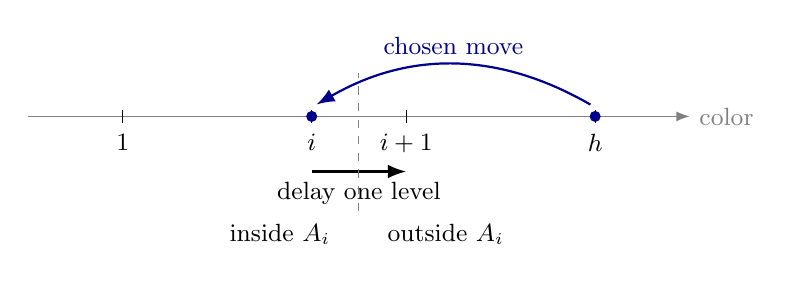
\begin{tikzpicture}[x=1.2cm,y=1cm,>=Latex,font=\small]
\draw[->,gray] (0,0) -- (7,0) node[right]{color};
\foreach \x/\lab in {1/{1},3/{i},4/{i+1},6/{h}} {
  \draw (\x,-.08) -- (\x,.08);
  \node[below] at (\x,-.1) {$\lab$};
}
\fill[blue!55!black] (3,0) circle (2pt);
\fill[blue!55!black] (6,0) circle (2pt);
\draw[->,thick,blue!55!black] (5.95,.15) to[bend right=30]
 node[above] {chosen move} (3.05,.15);
\draw[->,thick] (3,-.7) -- node[below]{delay one level} (4,-.7);
\draw[dashed,gray] (3.5,-1.2) -- (3.5,.55);
\node[anchor=east] at (3.3,-1.5) {inside $A_i$};
\node[anchor=west] at (3.7,-1.5) {outside $A_i$};
\end{tikzpicture}

\caption{The one-level delay in the reconstruction argument. A vertex
originally colored $h>i$ has been moved to $i$; delaying it to $i+1$
removes it from $A_i$ alone. At the same time $m_i$ decreases by one,
lowering the right side of \eqref{sel:feasibility} by $\varepsilon_i$.
Its membership in every other cumulative set $A_j$ stays fixed.
The drawing is schematic; $h$ may equal $i+1$.}
\label{fig:one-level-delay}
\end{figure}

\medskip
\noindent\textit{Counting the original colorings.}
Given $z$ and the profile, an original coloring $a$ is determined by
its changed vertices of each color $i$ in $z$, together with their
original colors $h>i$.  By \eqref{sel:changed-vertices}, the number
of possibilities is at most
\begin{equation}
\label{sel:encoding-bound}
  \prod_{i=1}^s
    \binom{|R_i|}{t_i}
    \binom{t_i}{(n_{ih})_{h>i}},
\end{equation}
where the second factor is a multinomial coefficient.
The sets $R_i$ may overlap and may contain vertices of other colors
in $z$.  Counting arbitrary subsets of them only adds possibilities
to \eqref{sel:encoding-bound}; every actual coloring has a unique
encoding of the indicated form.

For $t>0$, \eqref{sel:large-weight-bound} and
$\binom{n}{k}\le(en/k)^k$ give
\begin{equation}
\label{sel:entropy-bound}
  \prod_{i=1}^s\binom{|R_i|}{t_i}
  \le
  \prod_{i:t_i>0}\left(\frac{e\,2^i t}{t_i}\right)^{t_i}
  \le \prod_{i=1}^s(e\,4^i)^{t_i}.
\end{equation}
To see the last inequality, apply weighted AM--GM with weights
$\alpha_i=t_i/t$ on the positive rows:
\[
  \prod_{i:t_i>0}
     \left(\frac{2^{-i}}{\alpha_i}\right)^{\alpha_i}
  \le \sum_{i:t_i>0}2^{-i}\le1.
\]
Raising this inequality to the power $t$ yields exactly the second
inequality in \eqref{sel:entropy-bound}.  Rows with $t_i=0$
contribute a factor of one.

For each pair in the group, its probability and cost satisfy the
exact identity
\begin{equation}
\label{sel:likelihood}
  p^tP(a)=P(z)
      \prod_{i=1}^s\left(\frac p{\pi_i}\right)^{t_i}
      \prod_{i<h}\pi_h^{n_{ih}}.
\end{equation}
All color probabilities are positive.  Combining
\eqref{sel:encoding-bound}--\eqref{sel:likelihood}, the contribution
of a fixed $z$ and profile to the right side of
\eqref{sel:cover-cost} is at most
\begin{equation}
\label{sel:profile-contribution}
  P(z)\prod_{i=1}^s
  \left[
     \left(\frac{e\,4^i p}{\pi_i}\right)^{t_i}
     \binom{t_i}{(n_{ih})_{h>i}}
     \prod_{h>i}\pi_h^{n_{ih}}
  \right].
\end{equation}
The witness and the sets $R_i$ can depend on the full profile, but
none of that dependence remains in this bound.

For fixed row sums $t_1,\ldots,t_s$, we can consequently sum
\eqref{sel:profile-contribution} over all nonnegative integer
profiles with those row sums, including profiles that do not
occur.  The multinomial theorem gives, for each row,
\[
  \sum_{\substack{(n_{ih})_{h>i}\ge0\\
                   \sum_{h>i}n_{ih}=t_i}}
      \binom{t_i}{(n_{ih})_{h>i}}
      \prod_{h>i}\pi_h^{n_{ih}}
  =\left(\sum_{h>i}\pi_h\right)^{t_i}\le1.
\]
Finally, summing over all colorings $z$ uses $\sum_zP(z)=1$.
Thus the right side of \eqref{sel:cover-cost} is at most
\begin{equation}
\label{sel:tuple-sum}
  \sum_{\substack{t_1,\ldots,t_s\ge0\\
                   t_1+\cdots+t_s>0}}
       \prod_{i=1}^s
         \left(\frac{e\,4^i p}{\pi_i}\right)^{t_i}
  =
  \sum_{\substack{t_1,\ldots,t_s\ge0\\
                   t_1+\cdots+t_s>0}}
       \prod_{i=1}^s\left(\frac e{64^i}\right)^{t_i},
\end{equation}
where both sums run over integer tuples.
Put $\rho=\sum_{i=1}^s e/64^i$.  For a fixed total
$\ell=t_1+\cdots+t_s$, each monomial in
\eqref{sel:tuple-sum} occurs in the expansion of $\rho^\ell$ with
a multinomial coefficient at least one.  Since
\[
  \rho<\frac e{63}<\frac1{21},
\]
we obtain
\[
  \text{right side of \eqref{sel:cover-cost}}
  \le\sum_{\ell\ge1}\rho^\ell
  =\frac{\rho}{1-\rho}<\frac1{20}.
\]
Together with \eqref{sel:cover-cost}, this proves that the bad
probability is at most $1/10$.

For every nonbad coloring the same $H$ satisfies all inequalities
in \eqref{sel:simultaneous-capture}.  Since the colors are integers,
\[
  \sum_{x\in X}a(x)\lambda_H(x)
  =1+\sum_{i=1}^s\bigl(1-\lambda_H(A_i(a))\bigr)
  \le1+\sum_{i=1}^s2^{-i}\le2.
\]
This proves \eqref{sel:average-color} and completes the proof.
\end{proof}

\Needspace{12\baselineskip}
\section{Rounding a fractional cover}\label{sec:rounding}

We convert the color bound into independent numerical variables on the
vertices. Their means will be small, while the common member supplied by
Theorem~\ref{thm:multiscale-selector} will force a positive amount of
fractional-cover mass onto sets whose products are at least one. Comparing
the resulting lower and upper bounds on the same expectation completes
the proof. This conversion follows the selector-to-rounding approach
of Dubroff, Kahn, and Park~\cite[Section~2]{DKP2024} and
Pham~\cite[arXiv version~1, Section~3]{Pham2024}. In particular, the
equal distribution of a set's weight among its vertices in
\eqref{round:mass} is Pham's construction. The simultaneous color
bound supplies the additional control used here for arbitrary set sizes.

\begin{proof}[Proof of Theorem~\ref{thm:main}]
Put
\[
 D=256,\qquad B=512,\qquad C=25B^4.
\]
Let $r\in(0,1]$ and suppose that $g:2^X\to[0,1]$ satisfies
\begin{equation}\label{round:cover}
 \sum_{S\subseteq H}g(S)\ge1\quad(H\in\mathcal F),
 \qquad
 \sum_{S\subseteq X}g(S)r^{|S|}\le\frac12.
\end{equation}
Set $p=r/C$. We prove that $\mathcal F$ is $p$-small.

First observe that $g(\varnothing)\le1/2$, since its contribution to the
second sum in \eqref{round:cover} is $g(\varnothing)$. For each
$H\in\mathcal F$, define
\begin{equation}\label{round:mass}
 M_H=\sum_{\varnothing\ne S\subseteq H}g(S)
 \ge1-g(\varnothing)\ge\frac12,
 \qquad
 \lambda_H(x)=\frac1{M_H}
 \sum_{\substack{\varnothing\ne S\subseteq H\\x\in S}}
 \frac{g(S)}{|S|}\quad(x\in X).
\end{equation}
The function $\lambda_H$ vanishes off $H$ and is a probability mass
function: summing over $x$ counts each nonempty $S$ exactly $|S|$ times.

Suppose, for a contradiction, that $\mathcal F$ is not $p$-small.
Let $s$ be the largest nonnegative integer for which
\begin{equation}\label{round:scale}
 p\sum_{i=1}^sD^i\le\frac12.
\end{equation}
Such an integer exists: zero satisfies the restriction, and $p>0$ makes
the geometric sums unbounded. Apply
Theorem~\ref{thm:multiscale-selector} to these probability masses and this
choice of $s$. Thus the colors $a(x)$ are independent, with
\[
 \P(a(x)=i)=\pi_i=D^ip\quad(1\le i\le s),
 \qquad
 \P(a(x)=s+1)=\pi_{s+1}=1-p\sum_{i=1}^sD^i.
\]
With probability at least $9/10$, there is an $H\in\mathcal F$ such that
$\sum_x a(x)\lambda_H(x)\le2$. Denote this event by $\mathcal E$, and set
\begin{equation}\label{round:variables}
 Y_x=B^{4-a(x)},\qquad
 Z=\sum_{\varnothing\ne S\subseteq X}g(S)\prod_{x\in S}Y_x.
\end{equation}

Fix an outcome in $\mathcal E$ and a corresponding member $H$. Writing
$\overline a(S)=|S|^{-1}\sum_{x\in S}a(x)$ for nonempty $S$, we have
\[
 \frac1{M_H}\sum_{\varnothing\ne S\subseteq H}
 g(S)\overline a(S)
 =\sum_x a(x)\lambda_H(x)\le2.
\]
Apply Markov's inequality to the probability distribution
$g(S)/M_H$ on the nonempty subsets of $H$. It gives
\[
 \sum_{\substack{\varnothing\ne S\subseteq H\\
                  \overline a(S)\le4}}g(S)\ge\frac{M_H}{2}.
\]
For every set in this sum,
\[
 \prod_{x\in S}Y_x
 =B^{\,|S|(4-\overline a(S))}\ge1.
\]
Consequently $Z\ge M_H/2\ge1/4$ on $\mathcal E$. This holds for each
outcome, although the corresponding $H$ may depend on the coloring.
Since $Z$ is nonnegative everywhere,
\begin{equation}\label{round:lower}
 \E Z\ge\frac14\P(\mathcal E)\ge\frac9{40}.
\end{equation}

For the upper bound, maximality of $s$ gives
\[
 \frac12<p\sum_{i=1}^{s+1}D^i\le2pD^{s+1}.
\]
As $B\ge D$, it follows that
\begin{equation}\label{round:tail}
 B^{-(s+1)}\le D^{-(s+1)}<4p.
\end{equation}
The variables $Y_x$ are independent and identically distributed, and
their common mean $\mu$ satisfies
\begin{align}
 \mu
 &=B^4\left(p\sum_{i=1}^s(D/B)^i
            +\pi_{s+1}B^{-(s+1)}\right)\notag\\
 &\le B^4\left(p\sum_{i=1}^s2^{-i}+4p\right)
 \le5B^4p=\frac r5.\label{round:mean}
\end{align}
The same estimates hold when $s=0$, with the first sums empty.
Independence now yields
\begin{align}
 \E Z
 &=\sum_{\varnothing\ne S\subseteq X}g(S)\mu^{|S|}\notag\\
 &\le\sum_{\varnothing\ne S\subseteq X}g(S)(r/5)^{|S|}
 \le\frac15\sum_{\varnothing\ne S\subseteq X}g(S)r^{|S|}
 \le\frac1{10}.\label{round:upper}
\end{align}
Here the factor $1/5$ is valid because every set in the sum is
nonempty. The bounds \eqref{round:lower} and \eqref{round:upper}
contradict one another.

Thus $\mathcal F$ is $r/C$-small for every admissible $r>0$. At $r=0$,
the family $\mathcal F$ itself is a cover of cost zero, since
$\varnothing\notin\mathcal F$. Taking $r=q_f(\mathcal F)$, with this
last observation covering the case $q_f(\mathcal F)=0$, proves
\[
 q_f(\mathcal F)\le25\cdot512^4\,q(\mathcal F).
\]
\end{proof}

\section{A consequence for unions of two sets}\label{sec:consequence}

The comparison also strengthens a recent bound for sets that cannot be
covered by two members of a large class. For $\mathcal A\subseteq2^X$,
write $\mu_p(\mathcal A)=\P(X_p\in\mathcal A)$ and define
\[
 \operatorname{Bad}_2(\mathcal A)
 =\{S\subseteq X:S\nsubseteq A_1\cup A_2
                   \text{ for all }A_1,A_2\in\mathcal A\}.
\]
When $\mu_p(\mathcal A)>1/2$, Li's fractional discrete-convexity
theorem~\cite[Corollary~3.1]{Li2026} provides a fractional cover for this
family. Combining that input with Theorem~\ref{thm:main} gives the
following integral conclusion.

\begin{corollary}\label{cor:two-unions}
Let $X$ be a finite nonempty set, let $0<p<1$, and let
$\mathcal A\subseteq2^X$ satisfy $\mu_p(\mathcal A)>1/2$.
Set $C=25\cdot512^4$. There is a family $\mathcal G\subseteq2^X$ such
that
\[
 \operatorname{Bad}_2(\mathcal A)\subseteq\langle\mathcal G\rangle,
 \qquad
 \sum_{S\in\mathcal G}\left(\frac{p}{2C}\right)^{|S|}\le\frac12.
\]
In particular, $\operatorname{Bad}_2(\mathcal A)$ is
$(p/(2C))$-small. No monotonicity assumption on $\mathcal A$ is needed.
\end{corollary}

\begin{proof}
If $\operatorname{Bad}_2(\mathcal A)$ is empty, take
$\mathcal G=\varnothing$. Otherwise this is a nonempty increasing
family. It is proper because $\mathcal A$ is nonempty and hence
$\varnothing\notin\operatorname{Bad}_2(\mathcal A)$.
Li's theorem, in the covering formulation given by
Park~\cite[Theorem~3.4]{Park2026}, supplies a fractional cover of
$\operatorname{Bad}_2(\mathcal A)$ of cost at most $1/2$ at parameter
$p/2$. Its coefficients may be capped at one without affecting coverage
or increasing cost. Theorem~\ref{thm:main} therefore yields an integral
cover of cost at most $1/2$ at parameter $p/(2C)$.
\end{proof}

Park~\cite[Corollary~3.5]{Park2026} obtained the same conclusion with
smallness parameter
\[
 \frac{p}{K\max\{1,\log\log(1/p)\}}
\]
for a universal $K$. Corollary~\ref{cor:two-unions} removes the double
logarithmic loss
while retaining unions of two members and the covering budget $1/2$.

\begin{thebibliography}{99}

\bibitem{ALWZ2021}
Ryan Alweiss, Shachar Lovett, Kewen Wu, and Jiapeng Zhang,
\emph{Improved bounds for the sunflower lemma},
Annals of Mathematics \textbf{194} (2021), no.~3, 795--815.
\href{https://doi.org/10.4007/annals.2021.194.3.5}{doi:10.4007/annals.2021.194.3.5}.

\bibitem{BMM2022}
Witold Bednorz, Rafa{\l} Martynek, and Rafa{\l} Meller,
\emph{The suprema of selector processes with the application to positive
infinitely divisible processes},
preprint, 2022; version~3, 2026.
\href{https://arxiv.org/abs/2212.14636v3}{arXiv:2212.14636v3}.
\href{https://doi.org/10.48550/arXiv.2212.14636}{doi:10.48550/arXiv.2212.14636}.

\bibitem{DeMarcoKahn2015}
Bobby DeMarco and Jeff Kahn,
\emph{Note on a problem of M.~Talagrand},
Random Structures \& Algorithms \textbf{47} (2015), no.~4, 663--668.
\href{https://doi.org/10.1002/rsa.20559}{doi:10.1002/rsa.20559}.

\bibitem{DKP2024}
Quentin Dubroff, Jeff Kahn, and Jinyoung Park,
\emph{Note on a conjecture of Talagrand: expectation thresholds
vs.\ fractional expectation thresholds},
preprint, 2024.
\href{https://arxiv.org/abs/2412.00917v1}{arXiv:2412.00917v1}.
\href{https://doi.org/10.48550/arXiv.2412.00917}{doi:10.48550/arXiv.2412.00917}.

\bibitem{FischerPerson2025}
Thomas Fischer and Yury Person,
\emph{Some results on fractional vs.\ expectation thresholds},
Electronic Journal of Combinatorics \textbf{32} (2025), no.~3, Paper~P3.39.
\href{https://doi.org/10.37236/12611}{doi:10.37236/12611}.

\bibitem{FischerPerson2025further}
Thomas Fischer and Yury Person,
\emph{Further remarks on fractional vs.\ expectation thresholds},
preprint, 2025.
\href{https://arxiv.org/abs/2505.21782v1}{arXiv:2505.21782v1}.

\bibitem{FischerPerson2026random}
Thomas Fischer and Yury Person,
\emph{Fractional vs.\ expectation thresholds: random support case},
in 37th International Conference on Probabilistic, Combinatorial and
Asymptotic Methods for the Analysis of Algorithms (AofA~2026),
Leibniz International Proceedings in Informatics \textbf{381} (2026), 24:1--24:10.
\href{https://doi.org/10.4230/LIPIcs.AofA.2026.24}{doi:10.4230/LIPIcs.AofA.2026.24}.

\bibitem{FKNP2021}
Keith Frankston, Jeff Kahn, Bhargav Narayanan, and Jinyoung Park,
\emph{Thresholds versus fractional expectation-thresholds},
Annals of Mathematics \textbf{194} (2021), no.~2, 475--495.
\href{https://doi.org/10.4007/annals.2021.194.2.2}{doi:10.4007/annals.2021.194.2.2}.

\bibitem{FrankstonKahnPark2022}
Keith Frankston, Jeff Kahn, and Jinyoung Park,
\emph{On a problem of M.~Talagrand},
Random Structures \& Algorithms \textbf{61} (2022), no.~4, 710--723.
\href{https://doi.org/10.1002/rsa.21077}{doi:10.1002/rsa.21077}.

\bibitem{KahnKalai2007}
Jeff Kahn and Gil Kalai,
\emph{Thresholds and expectation thresholds},
Combinatorics, Probability and Computing \textbf{16} (2007), no.~3, 495--502.
\href{https://doi.org/10.1017/S0963548307008474}{doi:10.1017/S0963548307008474}.
\href{https://arxiv.org/abs/math/0603218v2}{arXiv:math/0603218v2}.

\bibitem{Li2026}
Chen Li,
\emph{On $p$-Spread Measures},
preprint, September~8, 2026.
\href{https://arxiv.org/abs/2609.08967v1}{arXiv:2609.08967v1}.

\bibitem{Park2026}
Jinyoung Park,
\emph{A dimension-free comparison between expectation thresholds and
fractional expectation thresholds},
preprint, September~13, 2026.
\href{https://arxiv.org/abs/2609.14681v1}{arXiv:2609.14681v1}.

\bibitem{ParkPham2024selector}
Jinyoung Park and Huy Tuan Pham,
\emph{On a conjecture of Talagrand on selector processes and a consequence
on positive empirical processes},
Annals of Mathematics \textbf{199} (2024), no.~3, 1293--1321.
\href{https://doi.org/10.4007/annals.2024.199.3.6}{doi:10.4007/annals.2024.199.3.6}.
\href{https://arxiv.org/abs/2204.10309v2}{arXiv:2204.10309v2}.

\bibitem{ParkPham2024threshold}
Jinyoung Park and Huy Tuan Pham,
\emph{A proof of the Kahn--Kalai conjecture},
Journal of the American Mathematical Society \textbf{37} (2024), no.~1, 235--243.
\href{https://doi.org/10.1090/jams/1028}{doi:10.1090/jams/1028}.

\bibitem{Pham2024}
Huy Tuan Pham,
\emph{A sharp version of Talagrand's selector process conjecture and an
application to rounding fractional covers},
in Proceedings of the 57th Annual ACM Symposium on Theory of Computing
(STOC~'25), ACM, New York, 2025, pp.~322--328.
\href{https://doi.org/10.1145/3717823.3718256}{doi:10.1145/3717823.3718256}.
Preprint version: \href{https://arxiv.org/abs/2412.03540v1}{arXiv:2412.03540v1}, 2024.

\bibitem{Pham2026}
Huy Tuan Pham,
\emph{A sharp version of Talagrand's selector process conjecture, with
applications to rounding fractional covers and Bernoulli Sudakov minoration},
expanded preprint, 2026.
\href{https://arxiv.org/abs/2412.03540v2}{arXiv:2412.03540v2}.
\href{https://doi.org/10.48550/arXiv.2412.03540}{doi:10.48550/arXiv.2412.03540}.

\bibitem{Talagrand2010}
Michel Talagrand,
\emph{Are many small sets explicitly small?},
in Proceedings of the Forty-Second ACM Symposium on Theory of Computing
(STOC~'10), ACM, New York, 2010, pp.~13--36.
\href{https://doi.org/10.1145/1806689.1806693}{doi:10.1145/1806689.1806693}.
\href{https://michel.talagrand.net/preprints/small.pdf}{Author's version}.

\end{thebibliography}

\end{document}
